\chapter{Einleitung}

%----------------------------------------------------------------------------------------

Die folgenden Kapitel beschreiben den Prozess, der nötig war um das Schloss
Rapperswil mittels Luftbilder als 3D-Modell zu rekonstruieren. Wir gehen hier
nicht auf die Evaluation der genutzten Software ein, dies folgt im nächsten Teil
dieser Dokumentation.

%----------------------------------------------------------------------------------------

\section{Erfassung des Schlosses mit Kamera-Drohne}

\label{workflow:drone}

Um Fotos des Schlosses von allen Winkeln zu erstellen, braucht man ein
ferngesteuertes Flugobjekt, wie \zb{} einen Multikopter. In unserem Fall wurden
die Fotos von Michael Suter (\url{http://lightmoment.ch/}) erstellt, der einen
Quadrokopter besitzt und damit freundlicherweise seine Piloten-Fähigkeiten unter
Beweis gestellt hat.

\subsection{Materialliste}

\begin{itemize}
	\item Quadrokopter: \textit{Team BlackSheep Discovery
		Pro}\footnote{\url{http://www.team-blacksheep.com/products/prod:discopro}}
	\item Kamera: \textit{GoPro Hero 4 Black}\footnote{\url{https://gopro.com/}}
	\item GPS Tracker: \textit{Fairphone
		FP1}\footnote{\url{https://www.fairphone.com/}} mit
		\textit{GeoTracker}
		App\footnote{\url{https://play.google.com/store/apps/details?id=com.ilyabogdanovich.geotracker}}
\end{itemize}

\subsection{Vorgehen}

Die maximale Flugzeit pro Akku beträgt 10--15 Minuten. Wir hatten zwei geladene
Akkus dabei und erreichten somit eine Flugzeit von 20--30 Minuten.

Die GoPro Kamera hatten wir so eingestellt, dass sie zwei mal pro Sekunde ein
Bild machte. Daraus ergaben sich dann etwa 2700 Fotos, was ca. 5.3 GiB
Bildmaterial entspricht.

Um Bewegungs-Unschärfe bei den Bildern zu vermeiden, ist es wichtig, dass der
Multikopter über eine Kamera-Stabilisierung verfügt. Dies ist bei der genutzten
TBS Discovery mit einem Gimbal (gyroskopische Mehrachsen-Stabilisierung)
gegeben.

Zur Aufzeichnung der GPS-Koordinaten haben wir ein Smartphone mit einer GPS
Tracking App auf dem Quadrokopter befestigt.

Mit dem Quadrokopter sind wir dann während einer halben Stunde mehrmals um das
Schloss herumgeflogen um Fotos von jedem Winkel zu erstellen. Auch den Innehof
haben wir mit dem Quadrokopter abgeflogen. Anschliessend sind wir noch zu Fuss
mit der Kamera in der Hand dem Pfad neben dem Schloss gefolgt um auch gutes
Bildmaterial von innerhalb des Tores zu erhalten.

\vspace{1\baselineskip}

\begin{figure}[H]
	\centering
	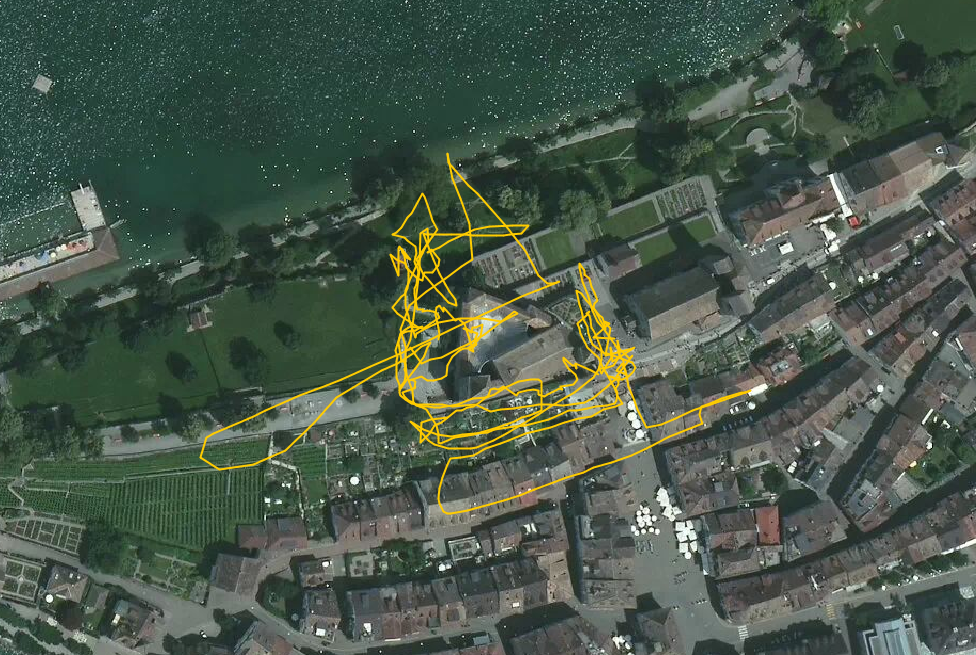
\includegraphics[width=\textwidth]{images/gpstrace_satellite.png}
	\caption{GPS Trace des Quadrokopters während der Erfassung.\\Bildmaterial:
		\copyright{} Bing Maps}
	\label{img:gpstrace-satellite}
\end{figure}

\begin{figure}[H]
	\centering
	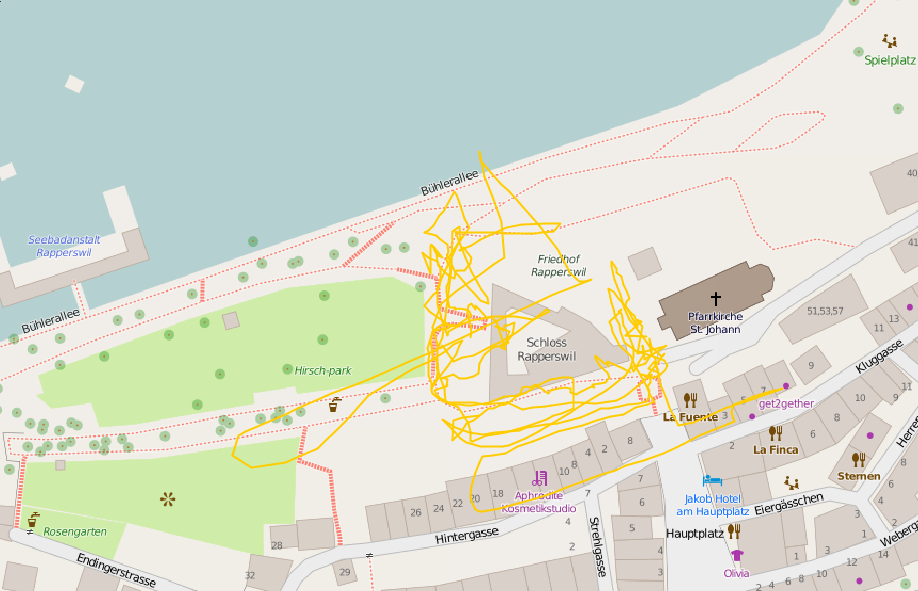
\includegraphics[width=\textwidth]{images/gpstrace_mapnik.png}
	\caption{GPS Trace des Quadrokopters während der Erfassung.\\Bildmaterial:
		\copyright{} OpenStreetMap Contributors}
	\label{img:gpstrace-mapnik}
\end{figure}

\subsection{Bildqualität}\label{workflow:erfassung:bildqualitaet}

Die GoPro Kamera ist für Sportaktivitäten entwickelt worden und hat daher ein
Weitwinkel-Objektiv ("<Fisheye">) eingebaut. Dies ist bestens geeignet um
beispielsweise beim Skifahren einen guten Überblick zu bewahren, für die
Rekonstruktion ist es aber eher nachteilig.

Ein weiterer Faktor ist die Kompression. Um viele Bilder auf der SD-Karte
speichern zu können, werden die JPEG-Bilder stark komprimiert. Die daraus
entstehenden JPEG-Artefakte können die Feature-Detection stören.

\marginpar{Das Raw-Format, auch Rohdaten- format genannt, bezeichnet eine Familie
von Dateiformaten für Digitalkameras, bei denen die Kamera die
Bildinfor- mationen nach der Digitalisierung direkt ohne weitere Bearbeitung auf
das Speichermedium schreibt. Bilder im Rohdatenformat werden gelegentlich auch
als "<Digitales Negativ"> bezeichnet.}

Idealerweise würde man daher zur Erfassung eine Spiegelreflex-Kamera mit
neutralem 35mm Objektiv verwenden und alle Bilder im Raw-Format abspeichern.
Diese können dann mit entsprechender Software ohne verlustbehaftete Kompression
in ein für die Photogrammetrie\-/Software nutzbares Format umgewandelt werden.

In unserem Fall waren wir aber durch die Tragfähigkeit des Quadrokopters
eingeschränkt und haben uns stattdessen dafür entschieden, die Bilder am
Computer mithilfe eines Linsenprofils in Photoshop
Lightroom\footnote{\url{http://www.photoshop.com/products/photoshoplightroom}}
zu entzerren.

Inzwischen gibt es zwar Photogrammetrie\-/Programme welche die GoPro
Linsenprofile direkt unterstützen. Nichtsdestotrotz gibt es sicher Kameras,
welche besser für solche Aufgaben geeignet sind als die GoPro.

\subsection{Learnings}

\begin{itemize}
	\item Die Jahreszeit war an sich gut gewählt, da die Bäume im Winter nicht
		belaubt sind, wodurch die Sicht auf das Schloss nicht eingeschränkt wird.
	\item Nachteilig war jedoch der Schnee auf den Dächern. Er überdeckte die
		Dachziegel und führte so bei der Feature-Erkennung zu schlechteren
		Ergebnissen.
	\item Die GoPro Kamera hat eine äusserst starke Linsen-Verzerrung. Eine Kamera
		mit neutraler Linse wäre vermutlich besser geeignet.
	\item Die JPEG Kompression ist möglicherweise störend. Eine Kamera mit
		Unterstützung für unkomprimierte Bilder (Raw-Format) würde vielleicht
		bessere Resultate liefern.
\end{itemize}

%----------------------------------------------------------------------------------------

\section{Nachbearbeiten des Bildmaterials}

\label{sec:image-correction}

Um wie im letzten Kapitel bereits besprochen, haben wir unsere Bilder mithilfe
von Photoshop Lightroom nachbearbeitet um die Linsenverzerrung herauszurechnen.

Das Linsenprofil der GoPro 4 wird seit Photoshop Lightroom 5.7 unterstützt. Die
Korrektur kann für alle Bilder gleichzeitig im Batch-Korrektur-Modus erfolgen.
Nach der Korrektur haben wir die Bilder mit JPEG-Qualitätsstufe 100 exportiert.

Als Open Source Alternative zu Photoshop Lightroom wäre noch
Hugin\footnote{\url{http://hugin.sourceforge.net/}} zu erwähnen, mit dem
ebenfalls Bilder entzerrt werden können. Wir haben jedoch kein vorbereitetes
Linsenprofil für die GoPro 4 gefunden und uns deshalb aus Zeitgründen für
Lightroom entschieden. Ein Linsenprofil könnte jedoch selber erstellt werden.
Anleitungen dazu gibt es
online\footnote{\url{http://hugin.sourceforge.net/tutorials/calibration/en.shtml}}.

TODO: https://github.com/racerxdl/goprocorrect

%----------------------------------------------------------------------------------------

\section{Erster Versuch: Pix4D}

Die erste von uns getestete Software war
Pix4D\footnote{\url{https://pix4d.com/}}. Dieses Programm wurde von einem
EPFL-Spinoff in der Westschweiz entwickelt. Während die Vollversion relativ
teuer ist (7'900 CHF), gibt es eine Testversion mit eingeschränktem
Funktionsumfang (keine GPU\-/Beschleunigung, kein Export), welche wir für
unseren ersten Versuch genutzt haben.

Da die Software damit wirbt, problemlos mit grossen Datenmengen umgehen zu
können, haben wir direkt mal alle 2700 Fotos hineingeladen und einen
Rekonstruktions-Prozess gestartet. (Da Pix4D direkt Unterstützung für die GoPro
Linse mitbringt, ist die Entzerrung übrigens optional. Wir haben in diesem
Schritt darauf verzichtet.)

Die Rekonstruktion dauerte auf einem Intel Core i7-4790K mit 16 GiB RAM etwas
über 52 Stunden. Das resultierende Modell war jedoch leider fehlerhaft. Wie man
auf der \autoref{img:pix4d} erkennen kann, wurde die Gasse neben dem Schloss
der Schlossmauer entlang schräg nach oben geführt. Zudem war im endgültigen
Ergebnis der Hauptturm doppelt vorhanden, einmal schräg versetzt.

\begin{figure}[H]
	\centering
	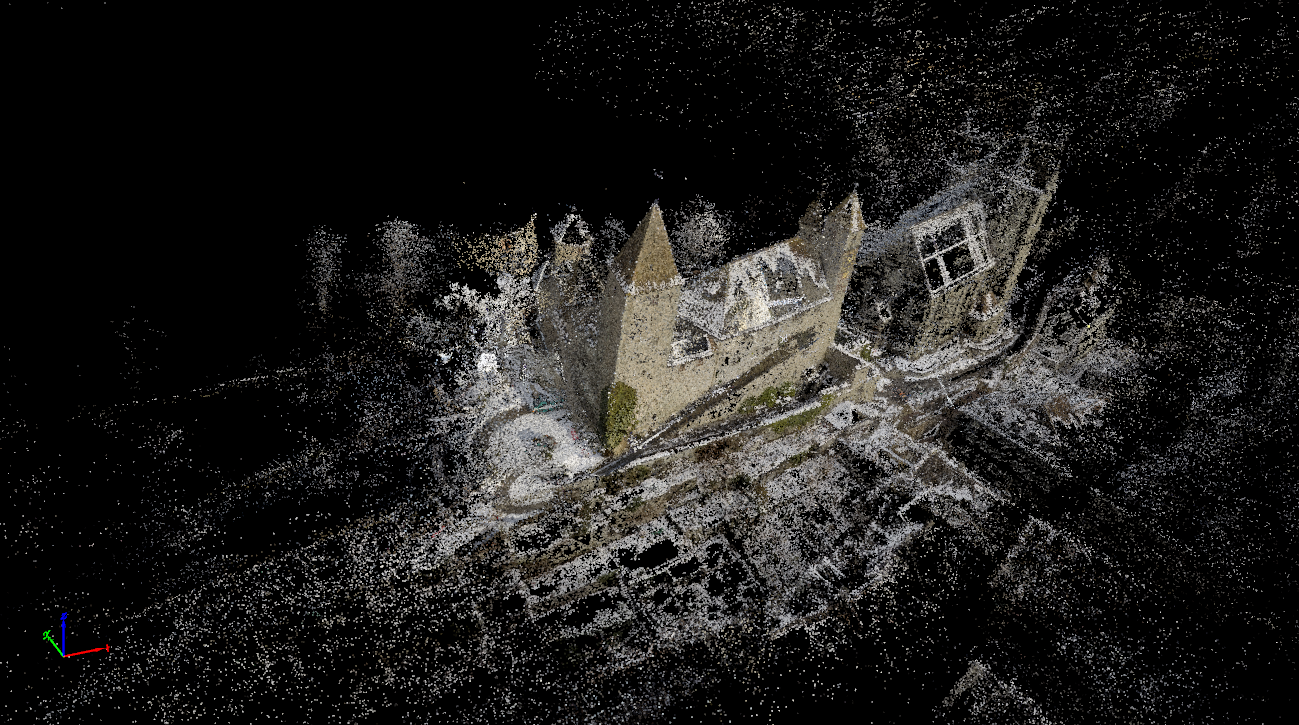
\includegraphics[width=\textwidth]{images/pix4d.png}
	\caption{Sparse Point Cloud in Pix4D}
	\label{img:pix4d}
\end{figure}

Unsere Vermutung ist, dass wir zu viele (teilweise qualitativ nicht
einwandfreie) Input-Daten verwendet hatten, so dass sich falsche Matches so weit
summiert haben, dass die Software sie als gültig betrachtet hat. Wir konnten
diese Hypothese aus Zeitgründen jedoch nicht verifizieren.

\subsection{Learnings}

\begin{itemize}
	\item Vermutlich ist es besser, die Anzahl Bilder auf die qualitativ
		hochwertigen zu reduzieren. Das senkt die Chance für fehlerhafte Matches.
	\item Ein Rekonstruktions-Algorithmus mit Unterstützung für sequentielle
		Bilder (oder Videos) könnte möglicherweise viel bessere Resultate liefern,
		da wiederum die Chance von falschen Matches reduziert wird.
	\item Möglicherweise war der zeitliche Abstand zwischen den Einzelbildern
		zu gross. Bei der Analyse zeitnaher Bilder würden wichtige Features
		stärker gewichtet, was eine Point-Cloud mit prozentual weniger
		falschen Punkten ergäbe.
\end{itemize}

%----------------------------------------------------------------------------------------

\section{Zweiter Versuch: VisualSFM}

Anstatt uns weiter mit Pix4D herumzuschlagen, haben wir den zweiten Versuch mit
VisualSFM\footnote{\url{http://ccwu.me/vsfm/}}\cite{wu:2011}\cite{wu:2015} unter
Linux gestartet. VisualSFM (Visual Structure From Motion, abgekürzt VSFM) wurde
von Changchang Wu im Jahr 2011 im Rahmen seines Postdoc Researches als Frontend
für die Photogrammetrie-Tools SiftGPU\cite{siftgpu07wu}, Multicore Bundle
Adjustment\cite{wu2011multicore}, CMVS\cite{Furu:2010},
PMVS\cite{Furu:2010:PMVS}, CMPMVS\cite{jancosek2011multi}, MVE\cite{FG-GCH2014},
SURE\cite{rothermel2012sure}, MeshRecon (und weitere) entwickelt. Der Quellcode
ist quelloffen, allerdings darf die Software gemäss ihrer proprietären Lizenz
ohne Kontaktaufnahme mit dem Autor nur zu akademischen und nonkommerziellen
Zwecken genutzt werden. Die verwendeten Komponenten sind teilweise unter einer
freien Lizenz\footnote{\url{https://www.fsf.org/licensing/}} veröffentlicht,
teilweise wie VSFM selbst nur für akademische und nonkommerzielle Zwecke
nutzbar.

\subsection{Installation}

Die Installation von VSFM kann etwas herausfordernd sein, deshalb haben wir im
\autoref{ch:installing-vsfm} die Installation unter Ubuntu 14.04 beschrieben.
Alternativ ist unter Arch Linux die Installation dank Paketen im Arch User
Repository\footnote{\url{https://aur.archlinux.org/packages/vsfm/}} relativ
einfach möglich.

\subsection{Konfiguration}

TODO: konfigurationsdatei, gpu beschleunigung, etc

\subsection{Vorgehen}

Beim Vorgehen haben wir uns an einem gut gemachten Tutorial auf YouTube
orientiert: \url{https://youtu.be/V4iBb_j6k_g}

Zuerst haben wir wie im \autoref{sec:image-correction} beschrieben die Fotos
einer Linsenkorrektur unterzogen. Anschliessend haben wir 571 Bilder für einen
Testlauf ausgewählt und in VSFM geladen. Bei der Auwahl haben wir darauf
geachtet, dass jeder Teil des Schlosses darin vertreten ist.

\begin{figure}[H]
	\centering
	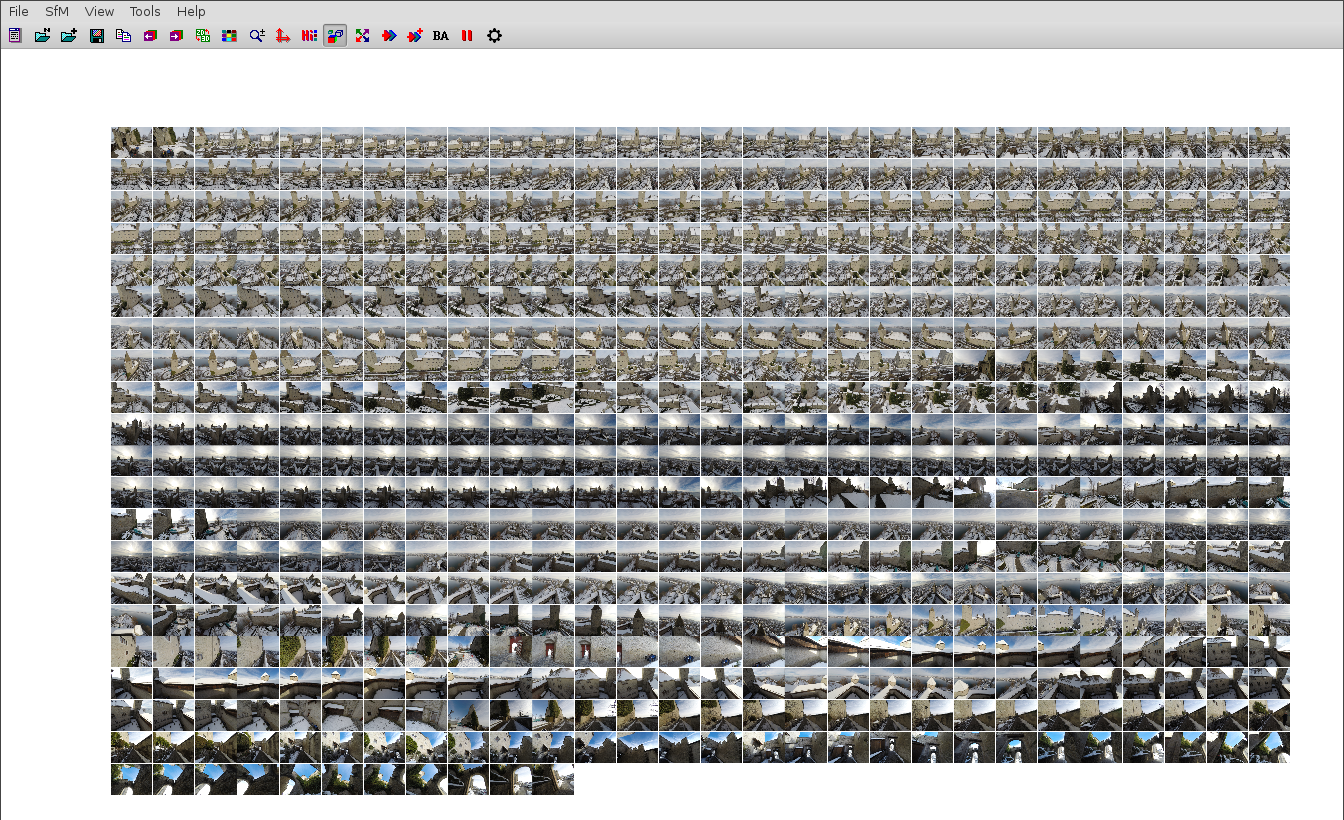
\includegraphics[width=\textwidth]{images/vsfm_thumbnails.png}
	\caption{Thumbnails in VSFM}
	\label{img:vsm_thumbnails}
\end{figure}

\noindent Für schnellere Resultate kann man optional die CUDA-Unterstützung unter \texttt{Tools > Enable GPU > Match using CUDA} aktivieren.

Mit einem Klick auf "<Compute Missing Matches">

\includegraphics[scale=0.75]{images/vsfm_icon_compute} wird die
Feature-Erkennung gestartet.

TODO screenshot

Nun kann mit einem Klick auf TODO die Rekonstruktion der Sparse Point Cloud
(siehe \autoref{photogrammetry:sparse-point-cloud}) beginnen. Man kann diese in
Echtzeit überwachen. Das Resultat lässt bereits die Umrisse des Schlosses
erahnen.

TODO screenshot

Als nächstes folgt die Schwerarbeit: Die Verdichtung der Punktwolke (siehe
\autoref{photogrammetry:dense-point-cloud}).

TODO screenshot


%----------------------------------------------------------------------------------------

\section{Mesh-Generierung}

TODO

%----------------------------------------------------------------------------------------

\section{Mesh-Bereinigung}

\label{workflow:mesh-cleanup}

Das Mesh ist nun bereit, sieht allerdings noch roh aus und weist viele
Unschönheiten auf. Diese müssen nun korrigiert werden. In unserem Fall geschah
dies von Hand.

Bei diesem Prozess wurden wir zu Beginn von der Firma Drei-De in Rapperswil
unterstützt. Sie übernahmen das initiale Mesh-Rework. Diese Arbeit hätte man
alternativ auch in MeshLab\footnote{\url{http://meshlab.sourceforge.net/}}
durchführen können.

Anschliessend haben wir die letzten Korrekturen mit der Software
Blender\footnote{\url{https://www.blender.org/}} durchgeführt.

\subsection{MeshLab}

MeshLab ist eine Software unter der GPL Lizenz, welches zur Ver- und Bearbeitung
von Meshes benutzt werden kann. Das Programm ist etwas gewöhnungsbedürftig und
lässt in der Bedienung zu Wünschen übrig, die eingebauten Funktionen sind jedoch
sehr mächtig.

\subsection{Blender}

Blender ist ebenfalls freie Software unter der GPL Lizenz. Das Programm kann
genutzt werden, um dreidimensionale Körper zu modellieren, sie zu texturieren,
zu animieren und zu rendern. Mit Hilfe von Blender wurden bisher schon mehrere
Kurzfilme produziert, darunter Sintel (2010, \cite{sintel}), Tears of Steel
(2012, \cite{tearsofsteel}) und
weitere\footnote{\url{http://archive.blender.org/features-gallery/movies/}}.

Wir haben primär mit den Modellier-Werkzeugen im sogenannten "<Sculpt Mode"> von
Blender gearbeitet. Diese sind der Arbeit mit Modelliermasse nachempfunden. Man
kann beispielsweise rauhe Stellen glätten, hervorstehende Flächen
"<hineindrücken">, etc. 

In unserem Fall mussten wir vor allem unebene Flächen glätten. Dies kann man mit
dem "<Flatten/Contrast"> Brush bei gedrückter \texttt{Shift}-Taste einfach
erledigen.

\begin{figure}[H]
	\centering
	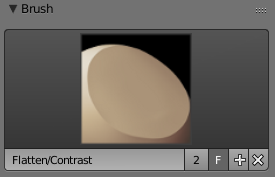
\includegraphics[width=0.4\textwidth]{images/blender_flatten_brush.png}
	\caption{Der Flatten/Contrast Brush}
	\label{img:blender_brush}
\end{figure}

Das fertige Mesh kann nun unter \texttt{File > Export > Stl (.stl)} ins STL
Format exportiert werden.

%----------------------------------------------------------------------------------------

\section{3D-Druck}

TODO

%----------------------------------------------------------------------------------------

\section{Resultate}

TODO
